% ============================================================
%  Competencia y Dependencia: México, China y las Nuevas
%  Rutas de Exportación hacia Estados Unidos
% ============================================================

\documentclass[11pt]{article}
% === Encoding & Language ===
\usepackage[utf8]{inputenc}
\usepackage[T1]{fontenc}        % only once
\usepackage[spanish,es-nodecimaldot]{babel}
\addto\captionsspanish{\renewcommand{\refname}{References}}
\addto\captionsspanish{\renewcommand{\abstractname}{Abstract}}

% === Fonts & Micro-typography ===
\usepackage{mathptmx}           % Times for text & math (from doc 1)
\usepackage{lmodern}            % fallback for non-Times glyphs
\usepackage{microtype}          % only once

% === Page Layout ===
\usepackage[top=2.5cm,bottom=2.5cm,left=3cm,right=3cm]{geometry}
% ↑ Chose doc 2's margins; replace with [margin=1in] if you prefer doc 1's

% === Math ===
\usepackage{amsmath,amssymb}    % merged; amssymb added from doc 2

% === Tables ===
\usepackage{booktabs}
\usepackage{multirow}
\usepackage{threeparttable}

% === Figures & Floats ===
\usepackage{graphicx}
\graphicspath{{../figures/}}
\usepackage{rotating}
\usepackage{float}
\usepackage{placeins}           % \FloatBarrier

% Float placement tuning
\setcounter{topnumber}{2}
\setcounter{bottomnumber}{1}
\setcounter{totalnumber}{3}
\renewcommand{\topfraction}{0.85}
\renewcommand{\bottomfraction}{0.5}
\renewcommand{\textfraction}{0.10}
\renewcommand{\floatpagefraction}{0.85}

% === Captions ===
\usepackage{caption}
\captionsetup{font=small, labelfont=bf, skip=8pt}

% === References ===
\usepackage[authoryear,round]{natbib}

% === Spacing & Paragraphs ===
\usepackage{setspace}
\usepackage{parskip}
\setlength{\parindent}{0pt}
\setlength{\parskip}{6pt}

% === Hyperlinks (load last, before soul) ===
\usepackage[hidelinks]{hyperref}

% === Drafting Aids ===
\usepackage{soul}

% === Drafting Aids ===
% --- Title -----------------------------------------------
\title{Competition and Dependence: Mexico, China, and the New Export
       Routes to the United States}

\author{
  Vladimir Márquez Stone\thanks{%
    Facultad de Economía, Universidad Nacional Autónoma de México (UNAM).
    Email: \href{mailto:vladimirmarquezst@comunidad.unam.mx}%
    {\texttt{vladimirmarquezst@comunidad.unam.mx}}.
    ORCID: \href{https://orcid.org/0009-0001-1187-6580}%
    {\texttt{0009-0001-1187-6580}}.}
  \and
  Seyka Sandoval\thanks{%
    Facultad de Economía, Universidad Nacional Autónoma de México (UNAM).
    Email: \href{mailto:seykasandoval@comunidad.unam.mx}%
    {\texttt{seykasandoval@comunidad.unam.mx}}.
    ORCID: \href{https://orcid.org/0000-0003-1552-9823}%
    {\texttt{0000-0003-1552-9823}}.}
}

\date{}  

\begin{document}
\maketitle    
% ============================================================
\begin{abstract}
This article analyzes the recent reconfiguration of Global Value Chains (GVC) among Mexico, China, and the United States in the context of the USMCA, nearshoring, and the global commercial tensions associated with the second China shock. Using bilateral trade data at the product level (HS6) from UN Comtrade from January 2016 to November 2024, we identify changes in direct competition between Mexico and China in the US market, as well as Mexico's persistent reliance on Chinese intermediate inputs. Using a difference-in-differences design with product and year-month fixed effects, we estimate that sectors where China held a higher pre-tariff share of US manufacturing imports experienced a differential increase of approximately 147\% in Mexican exports following the Section 301 tariffs ($\hat{\beta} = 1.474$, $t = 9.14$), without a corresponding rise in Chinese exports into Mexico, which rules out transit deflection as the dominant mechanism. Heterogeneity analysis reveals two distinct mechanisms: demand-side substitution in low-capacity sectors, and input sourcing restructuring with a reduction in Chinese component dependence in high-capacity sectors. In particular, the article documents the emergence of hybrid routes in which Mexico's export expansion to the United States coexists with the persistent integration of Chinese inputs, suggesting a partial reconfiguration of regional GVCs. We examine the productive and technological dependence on China and discuss the implications of these findings for Mexican industrial policy.

\medskip
\textbf{Keywords:} Nearshoring; Global Value Chains; Hybrid routes;
U.S.-China trade war; Mexican manufacturing; industrial policy.

\medskip
\textbf{JEL Classification:} F13, F14, F16, O25
\end{abstract}

% ============================================================
\renewcommand{\abstractname}{Resumen}
\begin{abstract}
Este artículo analiza la reconfiguración reciente de las Cadenas Globales de Valor (CGV) entre México, China y Estados Unidos en el contexto del T-MEC, del proceso de nearshoring y de las tensiones comerciales globales asociadas al denominado segundo shock de China. Utilizando datos bilaterales de comercio a nivel de producto (HS6) provenientes de UN Comtrade entre enero de 2016 y noviembre de 2024, identificamos cambios en los patrones de competencia directa entre México y China en el mercado estadounidense, así como en la dependencia de la manufactura mexicana respecto de insumos importados de China. Mediante un diseño de diferencias en diferencias con efectos fijos por producto y año-mes, estimamos que los sectores donde China concentraba una mayor participación previa en las importaciones estadounidenses registraron un crecimiento diferencial de aproximadamente 147\% en las exportaciones mexicanas tras los aranceles de la Sección 301 ($\hat{\beta} = 1.474$, $t = 9.14$), sin que ello se acompañara de un incremento en las exportaciones chinas hacia México, lo que descarta la hipótesis de deflexión de comercio. El análisis de heterogeneidad revela dos mecanismos distintos: en sectores de baja capacidad productiva previa, se observa sustitución por el lado de la demanda; en sectores de alta capacidad, una reestructuración de insumos, con una reducción de la dependencia de componentes chinos. En particular, el artículo documenta la emergencia de rutas híbridas en las que la expansión exportadora de México hacia Estados Unidos coexiste con una integración persistente de insumos chinos, lo que sugiere una reconfiguración parcial de las CGV regionales. Se enfatiza la dependencia productiva y tecnológica respecto de China y se discuten las implicaciones de estos resultados para la política industrial mexicana.

\medskip
\textbf{Palabras clave:} Nearshoring; Cadenas Globales de Valor; Rutas
híbridas; Guerra comercial EE.\,UU.--China; manufactura mexicana;
política industrial.

\medskip
\textbf{Clasificación JEL:} F13, F14, F16, O25
\end{abstract}

% ============================================================
\section{Introduction}

In 2023, Mexico surpassed China to become once again the largest exporter of goods to the United States. Although both North American countries already maintained high levels of economic integration, the trade war between the United States and China, initiated in 2017 through tariffs, export controls, and a policy of strategic decoupling, has redirected U.S. production linkages toward North America \citep{OropezaGarcia2024}. This phenomenon, termed nearshoring, has been defined as the regionalization of Global Value Chains (GVCs), initiated by cost differences and increasingly incorporating objectives of industrial policy, economic security, and strategic control of productive and technological assets \citep{Gereffi2025,Yellen2022,Xing2018}.

This transition has been marked by inconsistent negotiations and changes in the strategic objectives of successive US administrations \citep{Freund2025}. In July 2018, during Donald Trump's first term, the US government lifted the tariff exemption on Mexican products established under the North American Free Trade Agreement (NAFTA). In response, Mexico implemented retaliatory measures against various US products, affecting bilateral trade estimated at over three trillion dollars annually. In February 2018, the United States initiated a new trade war against Mexico, imposing tariffs of 25\,\% on all imports from Mexico and Canada, except for oil and energy, which would be subject to a 10\,\% tariff. In 2025, the United States' average effective tariff rate increased from 2.3 percent in 2024 to 13.1 percent in June 2025 \citep{Reinhart2025}.

As part of this process, the United States Trade Representative (USTR) has systematically resorted to unilateral trade policy instruments, particularly Sections 201 and 301 of the Trade Act of 1974, to impose tariffs and other restrictive measures. These provisions authorize President Donald Trump to take "all appropriate measures," including trade retaliation, to force the elimination of practices considered discriminatory by foreign governments \citep{RuizEstrada2025}. The contemporary use of these tools has been described as part of a US industrial policy aimed at reconfiguring production chains, protecting economic sectors, and preserving technological advantages amid geopolitical competition \citep{Ju2024}. China, for its part, has deployed an explicit state framework of industrial policy that directs subsidies, preferential financing, and tax incentives to sectors such as semiconductors, robotics, biotechnology, electric vehicles, and aerospace, articulating productive, technological, and geopolitical objectives in its participation in GVCs \citep{Autor2021,KehoeXu2025}.

Although this combination of industrial and trade policies, technological changes, and geopolitical competition has affected the Mexican manufacturing industry, the hybrid and multinational nature of GVCs makes it difficult to trace the effects of tariffs and trade wars on Mexican manufacturing. Mexico has lacked a comparable industrial strategy, operating as a functional space that both the United States and China employ to adjust their production and technological strategies. Mexican economic policy has prioritized FDI attraction and export-oriented manufacturing over the deliberate development of domestic productive and technological capabilities \citep{Gereffi2025}.

To evaluate Mexico's changing role within GVCs, it is necessary to understand how the dynamics of competition and dependence combine simultaneously along trade routes. The objective of this article is to analyze the reconfiguration of competition and dependence routes between Mexico and China with respect to exports of goods to the United States. In particular, we ask: in which sectors do Mexico and China compete most directly for the U.S. market? Which Mexican export sectors are most dependent on intermediate inputs from China to supply that market, and how are these hybrid routes configured? What recent changes have occurred in these routes as a result of the United States--Mexico--Canada Agreement (USMCA), nearshoring, or global trade tensions?

The article is organized as follows. Section~2 situates Mexico's participation in GVCs within the framework of the US-China trade dispute and the USMCA, reviewing the structural conditions that shape its productive and technological insertion. Section~3 describes the data and methodological strategy, including the construction of competition, dependence, and hybrid route indicators from bilateral product-level trade data, and the difference-in-differences design used to estimate the causal effect of Section~301 tariffs on Mexican and Chinese export flows. Section~4 presents the empirical results: we document the coexistence of direct competition between Mexico and China in the US market, estimate the differential expansion of Mexican exports in tariff-exposed sectors, and we characterize the persistence of Chinese input dependence across high- and low-capacity manufacturing sectors. Section~5 discusses the implications of these findings for trade and industrial policy, and examines the limitations of Mexico's current insertion strategy.

% ============================================================
\section{Background}

Mexico's participation in GVCs has been a fixed element of the country's
development strategy since the 1990s \citep{Sandoval2012}. Trade
liberalization was conceived as a strategy to attract foreign direct
investment (FDI), promote competitiveness, and diversify exports through
integration with the North American market. Since the early twenty-first
century, China's growing integration into world trade has shifted the
axis of GVCs toward East Asia, reducing the relative weight of North
American manufacturing and configuring a new interregional competition
\citep{Garrido2022}.

The current situation of Mexican manufacturing can be understood as the
result of trade policy decisions at the regional level and 
adjustments induced by structural transformations in the world economy.
\textit{Nearshoring}, understood as the relocation of productive
processes toward countries close to the destination market, has been
conceived as a space for promoting economic development, in
which the government articulates industrial and trade policy objectives,
and where productive linkages favor regionalization within the USMCA framework \citep{HernandezBenitez2023}. The
\textit{National Development Plan 2025--2030}, whose strategy centres on
expanding infrastructure and regional integration, contains explicitly
pro-industrial-policy and import-substitution language:

\begin{quote}
``Noteworthy is the formation of Plan México, an initiative that
envisages collaboration between the Government of Mexico and the private
sector, whose objective is to foster equitable and sustainable long-term
economic development, based on the use of our domestic market for our
own industry, thereby reducing unnecessary imports. This Plan seeks to
promote private investment, generate formal and quality employment,
increase national content in productive processes, simplify
administrative procedures, and combat poverty and inequality''
\citep[p.~17]{GobMex2025}.
\end{quote}

Public investment will continue "to play a central role in economic
development, oriented toward strategic projects that promote regional
industrialization and the strengthening of national content". The
relocation of investments is conceived as "an opportunity to consolidate
the country's productive and technological sovereignty'', with emphasis
placed on preserving fiscal orthodoxy around the autonomy of the Bank of
Mexico, balanced budgets, and the stability of public debt relative to
GDP \citep[pp.~17--18]{GobMex2025}.

While the Plan presents public investment as a central axis of the
development strategy and of technological capacity-building, the evidence
of its execution remains limited. Sectoral evidence suggests that Mexican
firms continue to participate in the least profitable segments of the value chain,
where technological spillovers and productive linkages are scarce
\citep{Sandoval2019,Basave2023,Basave2024,SandovalDuarte2025}.
On the other hand, facing trade tensions between Mexico and the United States, multinational firms operating in Mexico have deferred
investments and, in some cases, are considering relocating their
factories abroad \citep{Ando2024}, although such displacement is limited
for already-established investments \citep{Shih2020,Zhai2024}.

In this context, Mexico's trade bloc with the United States has
contributed to consolidating an institutional framework that structurally
limits trade integration beyond North America.\footnote{Within the USMCA region, there is a growing flow of
FDI, particularly in reinvestments, the consolidation of a dynamic
automotive and auto-parts sector, and the development of other strategic
sectors such as electronics, aerospace, and medical devices.} USMCA
introduced rules of origin and labor content requirements for the
Mexican manufacturing sector, and treaty clauses prohibit the signing of
trade agreements with states considered ``non-market'' economies, which in practice limits broad institutional rapprochement with China 
\citep{GomezRuiz2021}. 

This institutional lock-in also leaves Mexico structurally exposed to shifts in US trade policy \citet{RodriguezClare2025} estimate, using a dynamic model of trade and
reallocation with nominal wage rigidities, that US tariff increases and
retaliatory measures caused significant real income losses both in Mexico
and in other close US trading partners. \citet{FlachBaur2025} use a
quantitative trade model to simulate the impact of Trump's 25\,\% tariffs
on Mexico and Canada, and find that retaliatory measures will reduce
Mexico's manufacturing value added by up to 13\,\%, reflecting long-run
losses from tariff escalation, including efficiency losses, substitution
effects, declining exports, and a possible recession.

For Mexico, China is a central supplier of final goods, intermediate
inputs, and capital goods, while Mexican exports to China are relatively
scarce. In 2024, Mexico imported approximately 130 billion dollars (USD)
in goods from China, generating a significant and persistent trade
deficit. This imbalance can be interpreted as a growing technological
dependence of the Mexican manufacturing sector on Chinese-sourced inputs\citep{PerezSantilla2024}.
Analyses on Mexican manufacturing document a high
dependence on imported inputs, explained
endogenously by limited investment, particularly in science, technology,
and innovation (STI) \citep{Basave2024}, in labour force capacities
\citep{Basave2023}, and institutional environment \citep{KehoeXu2025}. 

This situation can be partially observed through the
``deterioration of the terms of trade'' hypothesis\footnote{This concept
derives from limited productive and export specialization, which
establishes an asymmetry between the high income-elasticity of imports
and the low income-elasticity of exports \citep{Prebisch1949}, exhibiting
a tendency toward structural balance-of-payments disequilibrium and
external vulnerability. The idea of ``structural external disequilibrium''
was the element that gave rise to the notion of the ``import substitution
industrialisation process'' \citep{NoyolaVazquez1957,Sunkel1958}, where
the disequilibrium ``is grounded in a basic diversity of productive
structures: specialization and heterogeneity characterize the peripheral
structure, in contrast to the diversification and homogeneity of the
centre'' \citep[p.~57]{Rodriguez2006}. This pattern of industrial
development generates limited horizontal diversification,
intersectoral complementarity, and vertical integration of productive
sectors, which do not permit rapid diversification of the peripheral countries
export supply, which tends to preserve its primary character for
prolonged periods \citep{Barcena2022}.}. The international value-added structure of trade is articulated by the design and control of strategic
technological and intermediate goods, produced or controlled through
ownership by firms located in the so-called \textit{core} countries,
while low-value-added manufacturing is located based on the network
\textit{leadership} design, in the non-core \textit{(peripheral)}
countries. \citep{LimaDuran2013,Garrido2022}.

For Mexico, the export of medium- and high-technology manufacturing has been extensively documented, alongside a high
dependence on imported inputs of greater technological complexity and a
specialization in assembly activities. This insertion character is reflected in the
low share of domestic value added in manufacturing exports and in the
predominance of backward linkages within GVCs
\citep{CastilloDeVries2018,Blyde2014}. In this sense, the deterioration
of the terms of trade manifests in the country's limited capacity to
generate significantly greater value added within the framework of its
insertion into the GVCs of the USMCA region.

Based on this diagnosis, \textit{Plan México} (2025) sets
out an import substitution strategy, particularly with respect to
China\footnote{Tariff policy, in the context of international trade
tensions, can be interpreted as an industrial policy instrument oriented
toward protecting or developing strategic sectors, incentivizing domestic
production, and reconfiguring participation in global value chains;
however, its effects are heterogeneous and depend on the productive and
institutional context \citep{Semieniuk2022,Qiu2019}.}, which seeks to increase productive
capacities, employment, worker compensation, and domestic value added, driven by
USMCA constraints and the second Trump administration tariff policy. Tariffs and trade policies more broadly can, under these conditions, operate as instruments for reconfiguring productive location and inducing substitution across GVCs \citep{Utar2023,Semieniuk2022}.

This perspective draws on the strategic trade literature, which moves beyond viewing tariffs as distortions and reconceptualizes them as instruments of industrial transformation. \citet{Rodrik2011} argues that tariffs can be instruments of ''policy
space'': for the design of industrial and technological policies
consistent with countries' own productive structures and levels of
development, even if this temporarily implies deviating from free
international competition. This revisits the models of
\citet{Krugman1983} and \citet{BranderSpencer1984,BranderSpencer1985,EatonGrossman1986}, which, departing
from perfect competition, argue that, since manufacturing is subject to
increasing returns, trade barriers can be absorbed by rents, allowing
domestic firms to gain scale, provided they manage to increase their
productivity and the government eventually withdraws protection, avoiding
rent capture by less efficient firms. Policies such as export subsidies
or selective restrictions can, under these conditions, improve national
welfare at the expense of other countries, in the same way that firms use
investment or R\&D to gain advantages in oligopolistic markets.

In this context, Plan México can be understood as Mexico's reaction to the second China shock, a policy initiative that seeks to implement trade and industrial policy actions as a mediator of US policies to combat trade surpluses that overflow traditional comparative advantage explanations and reflect, instead, a combination of industrial subsidies, directed credit to manufacturing firms, and financial mechanisms that prevent the appreciation of the Chinese currency and limit the absorption of imports
Although uncertainty persists regarding the causes of these imbalances, their most visible manifestation is the
massive expansion of Chinese exports \citep{Autor2016,Autor2021}. In response, the predominant reaction in recipient countries has been the imposition
of tariffs on Chinese goods, a measure supported by both protectionist
sectors and various political currents \citep{Freund2024}.

\citet{Pettis2024} asserts that trade imbalances during the second China shock cannot be understood solely through
comparative advantage, but are linked to macroeconomic configurations
such as the repression of domestic consumption, the transfer of income
toward sectors with increasing returns to scale, and the accumulation of
external surpluses. Pettis describes the misalignments
between savings, investment, and aggregate demand, as well as on the role
of the Chinese financial system and state in generating export
overcapacity. From this perspective, the ``China shocks'' influence the Mexican development trajectory by reinforcing
patterns of subordinate insertion into GVCs, where growth in export
volumes coexist with technological dependence and limited value-added capture \citep{OropezaGarcia2024}.

Plan México and the reactivation of industrial policy can be justified
as aimed at a transformation of manufacturing activity
consisting of a compositional shift that, due to the extraordinary
growth of Chinese export-oriented activities participating in global production
processes, widened the divergence with activities not participating in
such processes, oriented mainly toward the domestic market and locally
integrated, affecting their economic importance, while their degree of integration declined\citep{Xing2018}. \citet{KehoeXu2025} illustrate this contrast directly: China's upgrading along the value chain has been driven by technological sophistication, infrastructure investment, and R\&D promotion, while Mexico's growth has remained constrained by its dependence on exporting the same products as part of the North American supply chain.

Mexico's integration into GVCs is considered a pathway for manufacturing development; however, this assumption overlooks the hierarchical relations of production networks. Lead firms actively segment production, retain control over core technologies, and assign lower-value tasks to peripheral suppliers \citep{GereffiHumphreySturgeon2005,Sandoval2019}. Knowledge does not diffuse automatically; it is the object of dispute, negotiation, and often blockage. For countries integrated primarily as assembly centers, GVC participation can generate employment and export revenues without generating domestic technological capacities \citep{HumphreySChmitz2002}. This pattern describes with precision Mexico's insertion into the North American supply chain: sustained export growth concentrated in low-value-added segments, with persistent dependence on externally sourced inputs and technologies, a dependence that the nearshoring process reorganizes but does not structurally transform."

The two China shocks can be interpreted as a manifestation of structural
development problems in the case under study: asymmetric productive
specialization, technological dependence, and external constraints. The first shock reflected China's insertion as a low-cost manufacturing platform, which displaced industrial production in advanced and
semi-peripheral economies such as Mexico, deepening processes of
deindustrialization worldwide \citep{Autor2021}. The second China shock
is characterized by the expansion of productive capacity in medium- and
high-technology sectors, driven by active industrial policies, subsidies,
and directed credit, which intensifies global competition and reconfigures
value chains. As a result, China's development trajectory has shifted from
\textit{catching up} to \textit{forging ahead}, positioning itself as
one of the two central players in the world economy, competing for the
surplus of the dynamic economic sectors associated with the
electronics-computing sector and artificial intelligence.

% ============================================================
\section{Methods}
\subsection{Data}

We draw bilateral trade data from UN Comtrade
at the product level (HS6), restricted to manufacturing industries
(HS chapters 28--96). Three monthly flows are constructed for each sector~$s$:
exports from Mexico to the United States ($\text{MEX}{\to}\text{US}_{s,t}$),
exports from China to the United States ($\text{CHN}{\to}\text{US}_{s,t}$),
and imports into Mexico from China ($\text{CHN}{\to}\text{MEX}_{s,t}$).
We define two time windows: a pre-shock period
$\mathcal{T}_{0}$ (January 2016 -- December 2017) and a post-shock period
$\mathcal{T}_{1}$ (July 2018 -- November 2024), with 2018 treated as a
transition year. For any variable $Z_{s,t}$, the window average is

\begin{equation}
\overline{Z_{s}^{(\tau)}} =
\frac{1}{\left|\mathcal{T}_{\tau}\right|}
\sum_{t \in \mathcal{T}_{\tau}} Z_{s,t}, \qquad \tau \in \{0,1\}.
\end{equation}

Figure~\ref{fig:figura4} classifies each sector $s$ according to the
active presence of trade flows in the pre-tariff period, defined as a
monthly average value exceeding \$1{,}000, into five trade routes.
For each sector the log growth rates are computed as

\begin{align}
gX_{s} &= \log\!\left(\overline{\text{MEX}{\to}\text{US}_{s}^{(1)}}
+ \varepsilon\right)
- \log\!\left(\overline{\text{MEX}{\to}\text{US}_{s}^{(0)}}
+ \varepsilon\right), \\
gM_{s} &= \log\!\left(\overline{\text{CHN}{\to}\text{US}_{s}^{(1)}}
+ \varepsilon\right)
- \log\!\left(\overline{\text{CHN}{\to}\text{US}_{s}^{(0)}}
+ \varepsilon\right),
\end{align}

where $\varepsilon > 0$ avoids taking the logarithm of zero. A sector is
classified as a \textit{hybrid route} if the expansion of Mexican exports
to the US market coexists with a persistent or growing dependence on
Chinese inputs:

\begin{equation}
Hybrid_{s} = \mathbf{1}\!\left(gX_{s} > 0 \;\land\; gM_{s} \geq 0\right).
\end{equation}

\begin{figure}[H]
\centering
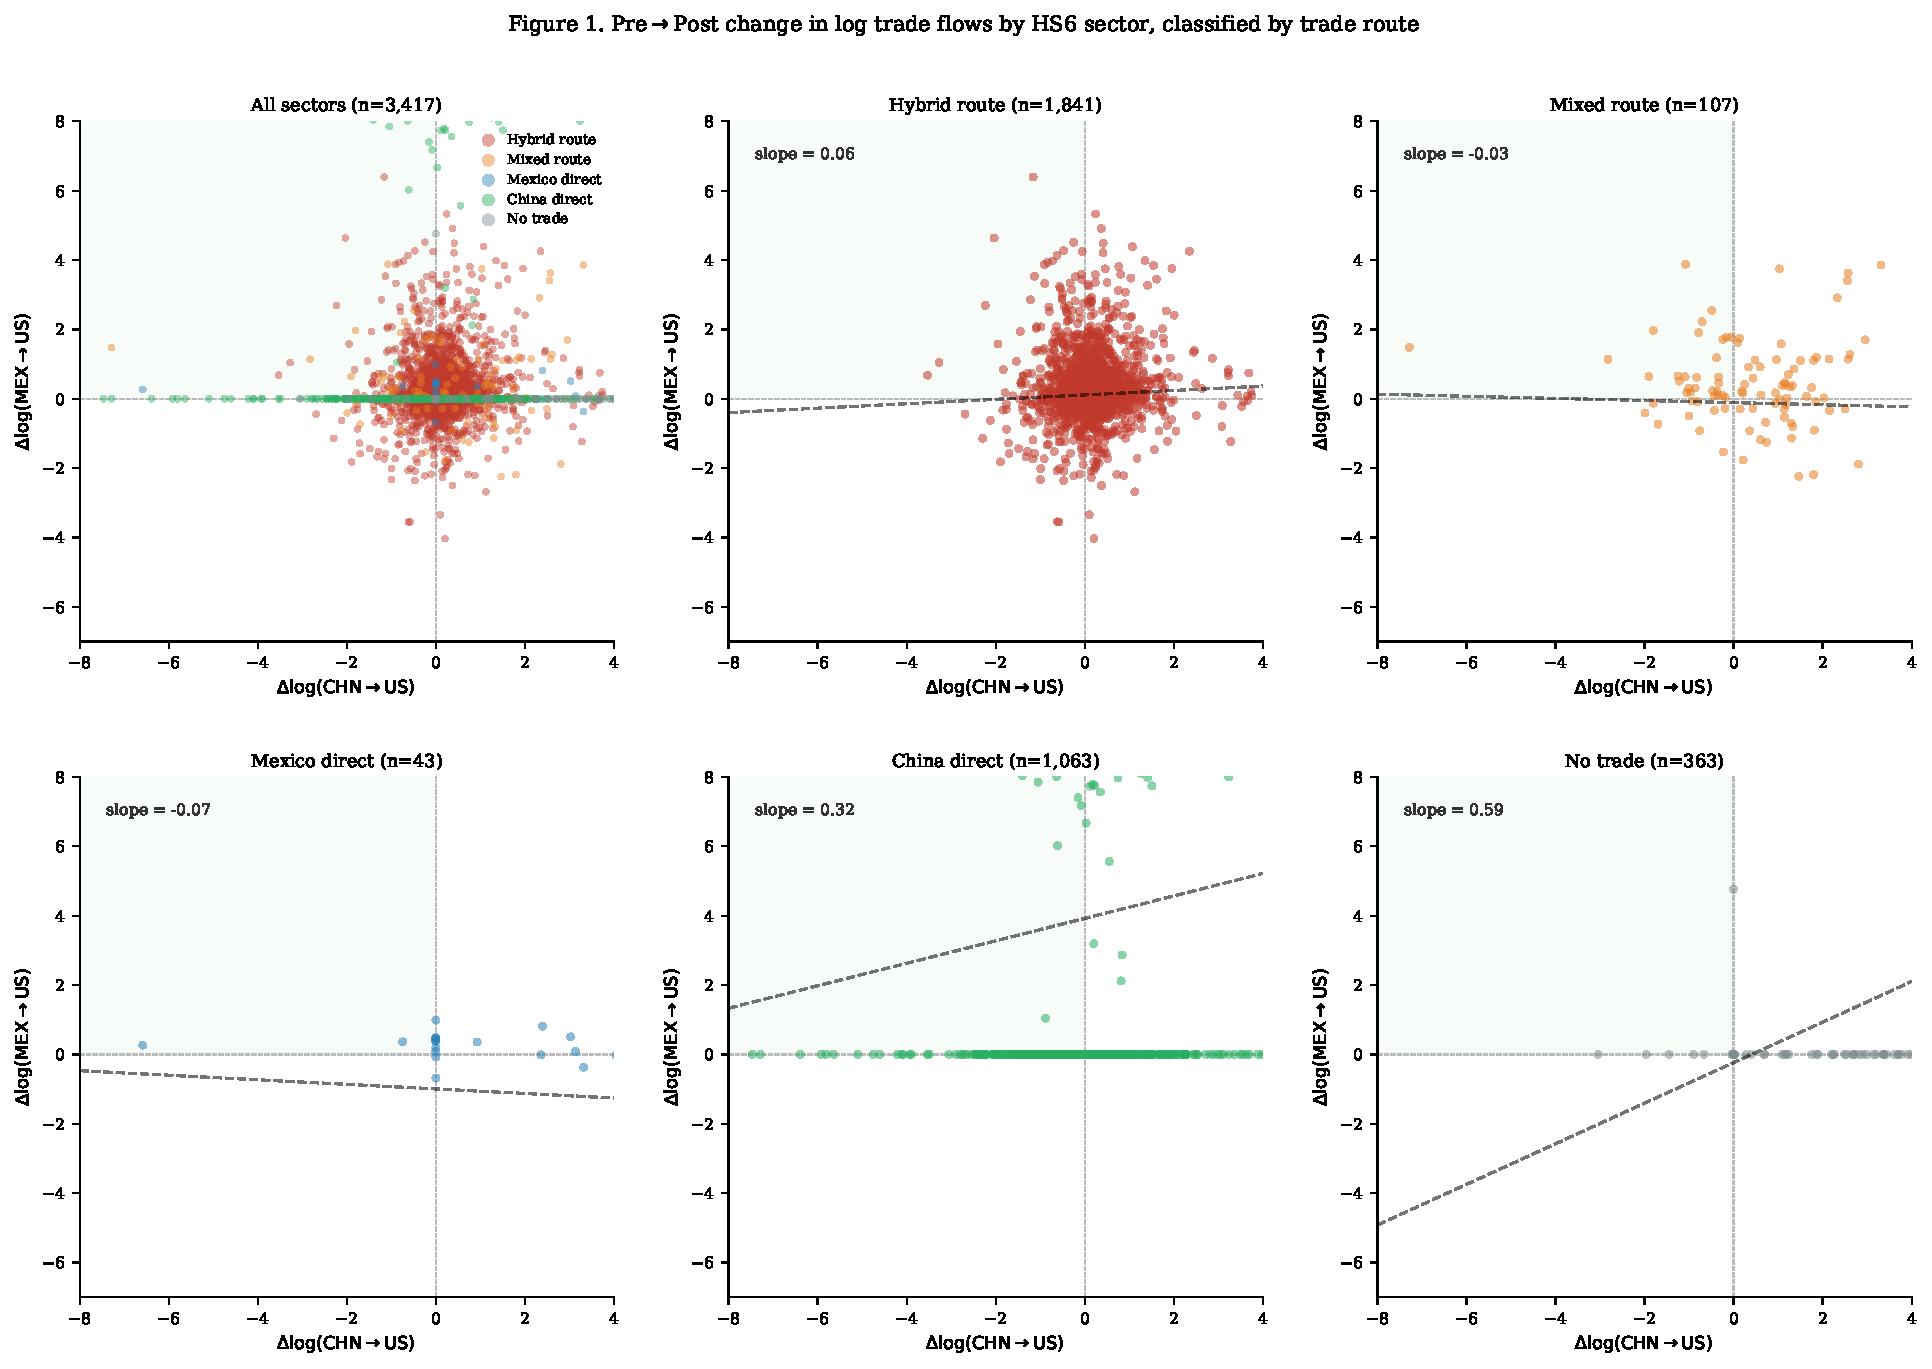
\includegraphics[width=\textwidth]{figure_1.pdf}
\caption{Pre/post shock change by HS6 category, disaggregated by trade
route. Authors' own elaboration.}
\label{fig:figura4}
\end{figure}

Figure~\ref{fig:figura4} plots $\Delta\log(\text{CHN}{\to}\text{US})$
against $\Delta\log(\text{MEX}{\to}\text{US})$ for each HS6 manufacturing
sector, disaggregated by pre-tariff trade route. In \textit{hybrid route}
sectors --- where all three bilateral flows were active before the
tariffs --- the slope is near zero (0.08), indicating that changes in
Chinese and Mexican export flows to the US were largely independent of
one another, consistent with tariff-induced demand substitution rather
than mechanical displacement. Sectors with only a Chinese pre-tariff US
route (\textit{China direct}, slope~$= 0.33$) and sectors with no prior
trade presence (\textit{no trade}, slope~$= 0.60$) show positive
co-movement driven by common sectoral shocks and the mechanical
amplification of small absolute changes in log space, respectively.
The \textit{Mexico direct} and \textit{mixed route} panels show slopes
close to zero, consistent with Mexican exporters responding to their own
demand conditions independently of Chinese performance.

\FloatBarrier

Table~\ref{tab:summary} presents summary statistics for the estimation
sample. Our panel covers 1,937 HS6 manufacturing product codes across 107
months from January 2016 to November 2024, and yields 207,259 sector-months
observations after restricting to codes present in all three trade flows.
Pre-tariff monthly exports from Mexico to the US average \$34.92M
at the HS6 level, compared to \$17.56M for Chinese exports to the US in the
same sectors. China's mean pre-tariff share of combined US imports (the
treatment variable) is 0.56, with substantial variation across sectors
(SD = 0.34), ranging from near-zero in sectors where Mexico historically
dominated to near-unity in sectors where Chinese goods faced little Mexican
competition.

\begin{table}[tbp]
\centering
\caption{Summary statistics}
\label{tab:summary}
\begin{threeparttable}
\renewcommand{\arraystretch}{0.85}

\textbf{Panel A: Panel structure} \\[4pt]
\begin{tabular}{lr}
\toprule
                              & Value \\
\midrule
Total observations            & 207,259 \\
Unique HS6 product codes      & 1,937 \\
HS2 sections                  & 41 \\
Months                        & 107 \\
Date range                    & Jan 2016 -- Nov 2024 \\
Post-tariff cutoff            & Jul 2018 (Section 301 List 1) \\
\bottomrule
\end{tabular}

\bigskip

\textbf{Panel B: Trade flow values (USD millions, non-zero HS6-month
observations)} \\[4pt]
\begin{tabular}{lrrrrrr}
\toprule
Flow & Mean & SD & P25 & Median & P75 & $n$ \\
\midrule
Mexico $\to$ US    & 34.92 & 189.66 & 0.34 &  2.20 & 12.45 & 131,644 \\
China $\to$ Mexico &  2.28 &  11.24 & 0.06 &  0.30 &  1.16 & 172,151 \\
China $\to$ US     & 17.56 & 109.26 & 0.31 &  1.83 &  8.55 & 192,989 \\
\bottomrule
\end{tabular}

\bigskip

\textbf{Panel C: Treatment variable --- China's pre-tariff US import
share} \\[4pt]
\begin{tabular}{lrrrrrr}
\toprule
 & Mean & SD & P25 & Median & P75 & $n$ \\
\midrule
TreatShare$_s$ & 0.559 & 0.337 & 0.236 & 0.599 & 0.892 & 207,259 \\
\bottomrule
\end{tabular}

\bigskip

\textbf{Panel D: Monthly aggregate exports, pre- and post-tariff (USD
billions)} \\[4pt]
\begin{tabular}{lrrr}
\toprule
Period & Mexico $\to$ US & China $\to$ US & China $\to$ Mexico \\
\midrule
Pre-tariff (2016--2017)          & 37.78 & 28.88 & 2.39 \\
Post-tariff (Jul 2018--Nov 2024) & 44.48 & 32.64 & 4.14 \\
Change (\%)                      & +17.6 & +13.0 & +73.2 \\
\bottomrule
\end{tabular}

\bigskip

\textbf{Panel E: Productive capacity split} \\[4pt]
\begin{tabular}{lr}
\toprule
 & HS6 codes \\
\midrule
High capacity (pre-tariff MEX$\to$US $\geq$ \$0.82M/month) & 969 \\
Low capacity  (pre-tariff MEX$\to$US $<$  \$0.82M/month)  & 968 \\
\bottomrule
\end{tabular}

\begin{tablenotes}[flushleft]
\footnotesize
\item \textit{Notes:}
Panel~A restricts to HS6 codes present in all three bilateral trade flows.
Panel~B reports USD millions for non-zero HS6-month observations; structural non-trading zeros are retained in the regression.
Panel~C defines treatment as China's share of combined China$+$Mexico manufacturing imports to the US, averaged over 2016--2017.
Panel~D reports simple monthly averages across all panel HS6 codes.
Panel~E splits at the median pre-tariff Mexico$\to$US export level
(\$0.82M/month).
All values from UN Comtrade; manufacturing defined as HS2 sections 28--30,
32--34, 38--40, 54--64, 72--80, and 84--96.
December months are included in Panels~B--D but excluded from regressions
to remove Comtrade reporting issues.
\end{tablenotes}

\end{threeparttable}
\end{table}

Figure~\ref{fig:aggregate_trends} documents the aggregate trends of the
three flows indexed to the 2016--2017 baseline. Total Mexican manufacturing
exports to the US reached approximately 48\% above their pre-tariff level
by 2024, while Chinese exports to the US in the same sectors were only 3\% above baseline. Chinese exports to Mexico,
our deflection diagnostic grew substantially, reaching 116\% above
baseline, but the composition, concentrated in intermediates rather than
finished goods, indicates supply chain deepening rather than
transit deflection. These descriptive patterns motivate the
identification strategy.

\begin{figure}[tbp]
  \centering
  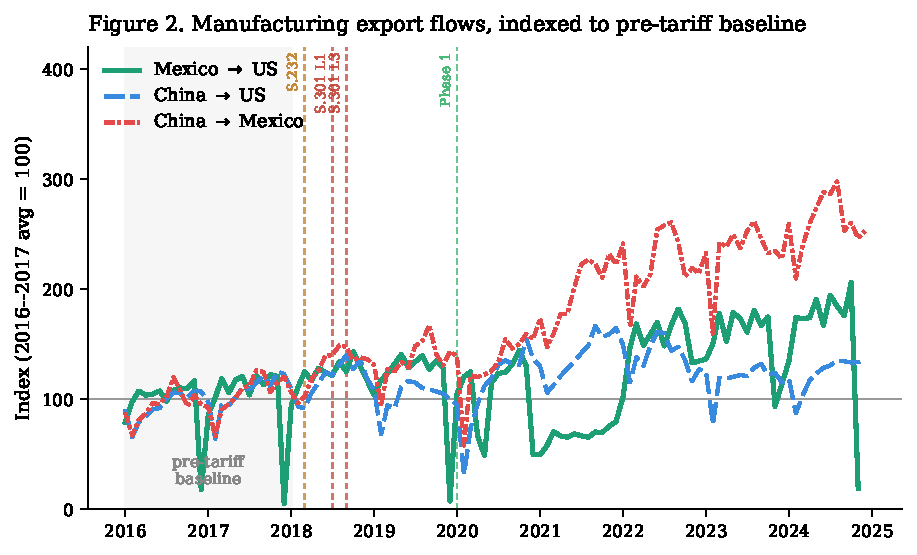
\includegraphics[width=0.75\textwidth, trim=0 10pt 0 0, clip]{figure_2.pdf}
  \caption{Manufacturing export flows, indexed to pre-tariff baseline}
  \label{fig:aggregate_trends}
  \vspace{4pt}
  {\footnotesize\textit{Notes:} Monthly FOB values (USD) for manufacturing
  HS6 product codes across three bilateral trade flows: Mexico to the US
  (solid), China to the US (dashed), and China to Mexico (dash-dot).
  Index equals 100 at the 2016--2017 average. Vertical markers denote key
  policy events: Section 232 steel and aluminum tariffs (Mar 2018),
  Section 301 List 1 (Jul 2018), Section 301 List 3 (Sep 2018), and the
  US--China Phase One deal (Jan 2020). Shaded region is the pre-tariff
  baseline period. Source: UN Comtrade.\par}
\end{figure}

% ─────────────────────────────────────────────────────────────────────────────
\FloatBarrier
\subsection{Pre-trends validation}
% ─────────────────────────────────────────────────────────────────────────────

A credible difference-in-differences design requires that sectors with
high and low Chinese pre-tariff US market share were on parallel
trajectories before the tariff shock. Figure~\ref{fig:es_mex_us} presents
the event study coefficients from estimating equation~\eqref{eq:es} over a
24-month pre-period and 30-month post-period window, with December months
excluded to remove Comtrade reporting issues. Formally, we estimate:

\begin{equation}
\log(1 + \mathrm{MEX\text{-}US}_{s,t}) =
  \alpha_s + \alpha_t +
  \sum_{k \neq -1} \beta_k
    \bigl( \mathrm{TreatShare}_s \times \mathbf{1}[t = k] \bigr)
  + \varepsilon_{s,t}
\label{eq:es}
\end{equation}

where all coefficients are normalized to zero at the pre-period mean.
The pre-period coefficients fluctuate around zero without trend
(pre-period mean $= 0.00$, SD $= 0.27$), providing no evidence of
differential pre-trends between high- and low-exposure sectors.
The post-period coefficients are initially close to zero and begin to
rise from approximately month $+15$ onward, indicating
gradual production relocation rather than an immediate mechanical response.

The corresponding event study for the deflection outcome
(Figure~\ref{fig:es_chn_mex}) shows a flat pre-period followed by a
persistent negative shift beginning around month $+8$ and deepening
through 2022--2024. This pattern rules out immediate transit deflection,
which would predict a positive post-period jump, and suggests supply chain restructuring away from Chinese inputs, as Mexican production expands.

\begin{figure}[tbp]
  \centering
  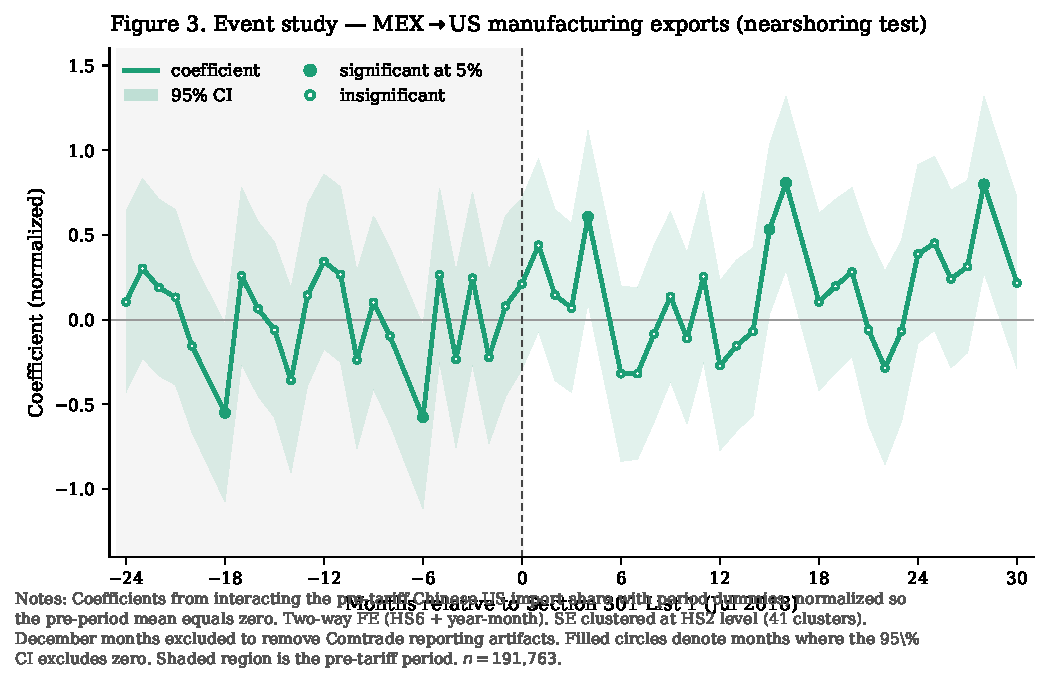
\includegraphics[width=0.75\textwidth, trim=0 60pt 0 0, clip]{figure_3.pdf}
  \caption{Event study --- MEX$\to$US manufacturing exports (nearshoring
           test)}
  \label{fig:es_mex_us}
  \vspace{2pt}
  {\footnotesize\textit{Notes:} Coefficients from interacting the
  pre-tariff Chinese US import share with period dummies, normalized so
  the pre-period mean equals zero. Two-way fixed effects (HS6 $+$
  year-month). Standard errors are clustered at the HS2 level (41 clusters).
  December months are excluded to remove Comtrade reporting issues.
  Filled circles denote months where the 95\% confidence interval
  excludes zero. The shaded region is the pre-tariff period.
  $n = 191{,}763$.\par}
\end{figure}

\begin{figure}[tbp]
  \centering
  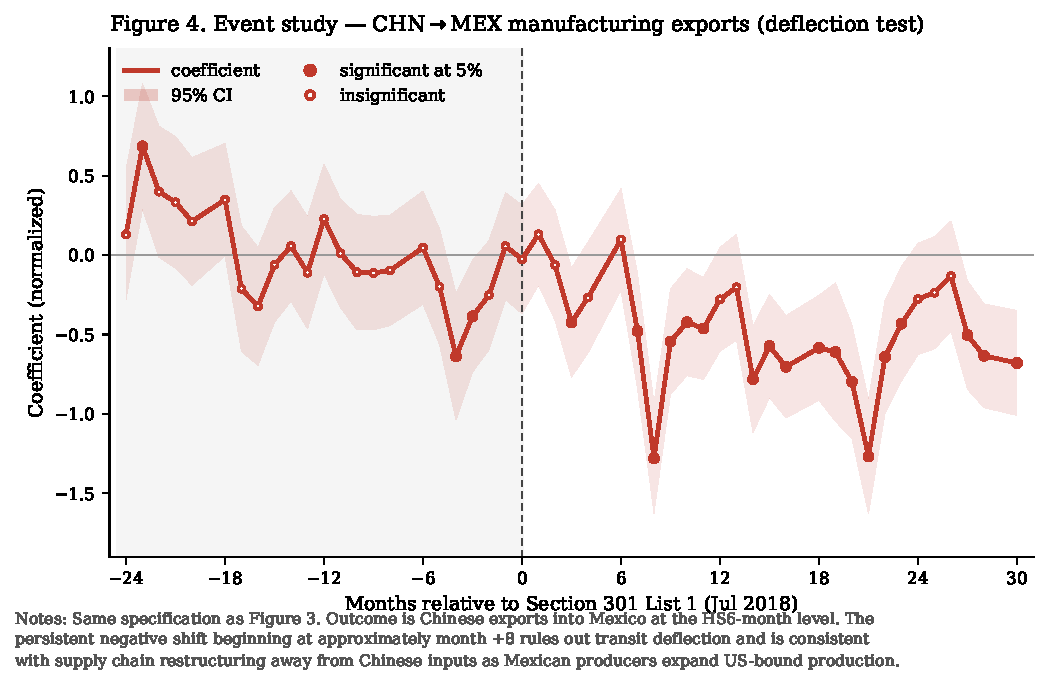
\includegraphics[width=0.7\textwidth, trim=0 60pt 0 0, clip]{figure_4.pdf}
  \caption{Event study --- CHN$\to$MEX manufacturing exports (deflection
           test)}
  \label{fig:es_chn_mex}
  \vspace{4pt}
  {\footnotesize\textit{Notes:} Same specification as Figure~\ref{fig:es_mex_us}.
  The outcome variable is Chinese exports into Mexico at the HS6-month
  level. The statistically significant negative shift beginning at
  approximately month $+8$ rules out transit deflection and indicates
  supply chain restructuring away from Chinese inputs as Mexican producers
  expand US-bound production.\par}
\end{figure}

% ─────────────────────────────────────────────────────────────────────────────
\FloatBarrier
\section{Results}
% ─────────────────────────────────────────────────────────────────────────────

Table~\ref{tab:main} presents the main regression results from estimating
the two-equation system. All specifications include HS6 product fixed
effects and year-month fixed effects, absorbing time-invariant sector
characteristics and all aggregate shocks common to manufacturing exports
in a given month. Standard errors are clustered at the HS2 section level
(41 clusters). Formally, we estimate:

\begin{align}
\log(1 + \mathrm{MEX\text{-}US}_{s,t}) &=
  \alpha_s + \alpha_t +
  \beta\,(\mathrm{TreatShare}_s \times \mathrm{Post}_t)
  + \varepsilon_{s,t}
  \label{eq:nearshoring} \\[6pt]
\log(1 + \mathrm{CHN\text{-}MEX}_{s,t}) &=
  \alpha_s + \alpha_t +
  \gamma\,(\mathrm{TreatShare}_s \times \mathrm{Post}_t)
  + \varepsilon_{s,t}
  \label{eq:deflection}
\end{align}

\noindent where $s$ indexes HS6 product codes and $t$ indexes year-months.
$\alpha_s$ are HS6 product fixed effects absorbing all time-invariant
sector characteristics. $\alpha_t$ are year-month fixed effects absorbing
aggregate shocks common to all sectors in a given month.
$\mathrm{TreatShare}_s$ is China's share of combined China$+$Mexico
manufacturing imports to the US averaged over the pre-tariff period
(2016--2017), measuring the intensity of competitive displacement.
$\mathrm{Post}_t = 1$ from July 2018 onward (Section 301 List 1).
The coefficient $\beta$ in equation~\eqref{eq:nearshoring} tests whether
Mexican exports to the US rose differentially in sectors most exposed to
Chinese displacement (nearshoring). The coefficient $\gamma$ in
equation~\eqref{eq:deflection} tests whether Chinese exports into Mexico
rose in the same sectors (deflection). Both equations are estimated
separately via OLS with the two-way fixed effects absorbed through
iterative demeaning.

\begin{table}[tbp]
\centering
\caption{Main results: effect of Chinese tariff exposure on Mexican and
         Chinese manufacturing trade flows}
\label{tab:main}
\begin{threeparttable}

\begin{tabular}{lcc}
\toprule
 & (1) & (2) \\
 & MEX$\to$US & CHN$\to$MEX \\
 & (nearshoring test) & (deflection test) \\
\midrule
TreatShare$_s \times$ Post$_t$
    & $1.474^{***}$ & $-0.279$ \\
    & $(0.161)$     & $(0.183)$ \\[6pt]
\midrule
HS6 fixed effects        & Yes & Yes \\
Year-month fixed effects & Yes & Yes \\
Observations             & 247,170 & 247,170 \\
HS6 codes                & 1,937 & 1,937 \\
HS2 clusters             & 41 & 41 \\
\bottomrule
\end{tabular}

\begin{tablenotes}[flushleft]
\footnotesize
\item \textit{Notes:}
OLS estimates with two-way fixed effects (HS6 product and year-month),
absorbed via iterative demeaning.
Outcome in column~(1) is $\log(1 + \mathrm{MEX}\to\mathrm{US}_{s,t})$
and in column~(2) is $\log(1 + \mathrm{CHN}\to\mathrm{MEX}_{s,t})$.
TreatShare$_s$ is China's share of combined China$+$Mexico manufacturing
imports to the US, averaged over 2016--2017.
Post$_t = 1$ from July 2018 onward (Section 301 List 1).
Standard errors in parentheses, clustered at the HS2 section level.
Observation counts reflect non-zero trade flow observations after
within-transformation.
$^{***}p < 0.01$.
\end{tablenotes}

\end{threeparttable}
\end{table}

\textit{Equation~\eqref{eq:nearshoring} --- Nearshoring test.}
Column~(1) reports the effect of Chinese tariff exposure on Mexican
exports to the US. The coefficient $\hat{\beta}$ on
TreatShare$_s \times$ Post$_t$ is 1.474 (SE = 0.161, $t = 9.14$,
$p < 0.01$). Sectors where China held a one-unit higher pre-tariff share
of US manufacturing imports saw approximately 147\% more growth in log
Mexican exports after July 2018, relative to sectors where Mexico already
dominated. This estimate is robust across
specifications.

\textit{Equation~\eqref{eq:deflection} --- Deflection test.}
Column~(2) reports the parallel equation for Chinese exports into Mexico.
The coefficient $\hat{\gamma}$ is $-0.279$ (SE = 0.183, $t = -1.52$),
which is negative but statistically insignificant. In sectors most
displaced from the US market, Chinese exports into Mexico did not
rise, the opposite of what transit deflection would
predict. This constitutes the paper's core falsification result.

Taken together, the two equations point to a nearshoring mechanism:
sectors where Chinese goods lost US market access saw more Mexican exports
to the US and simultaneously showed no increase in Chinese goods flowing
into Mexico. The joint pattern is inconsistent with the null of no
adjustment and the alternative of transit deflection.

% ─────────────────────────────────────────────────────────────────────────────
\FloatBarrier
\subsection{Heterogeneity by productive capacity}
% ─────────────────────────────────────────────────────────────────────────────

The aggregate estimates mask heterogeneity in the adjustment
mechanism. If nearshoring reflects production relocation to
Mexico, the response should differ by Mexico's pre-existing
productive capacity in each sector, both because established Mexican
manufacturers can more rapidly absorb displaced demand, and because
capacity is a proxy for supply chain readiness. Table~\ref{tab:heterogeneity} splits the sample at the median pre-tariff
MEX$\to$US export level (\$0.82M per month) as a measure of Mexico's
pre-existing productive capacity. The results reveal two distinct patterns

In \textit{low-capacity sectors}, those where Mexico had minimal
pre-tariff export presence, the nearshoring coefficient is large and
significant ($\beta = 1.399$, $t = 5.56^{***}$), while the deflection
coefficient is negative but insignificant ($\beta = -0.234$,
$t = -1.06$). Mexican exports surged in precisely the sectors where China
was most displaced, without a corresponding rise in Chinese goods entering
Mexico. This is consistent with new entry, demand capture, or rapid
capacity expansion by Mexican manufacturers responding to 
opportunities opened by the tariffs.

In \textit{high-capacity sectors}, those where Mexico already had
established export positions, the nearshoring coefficient is positive
but statistically insignificant ($\beta = 0.388$, $t = 1.46$), while the
deflection coefficient is large and highly significant
($\beta = -1.545$, $t = -4.91^{***}$). Established Mexican manufacturers
show no additional export surge, but the fall in Chinese
imports into Mexico suggests they actively restructured their input
sourcing, reducing reliance on Chinese components as they deepened
domestic or non-Chinese supply chains.

We interpret the following two mechanisms: Low-capacity sectors experienced
demand-side substitution: Mexican producers captured the markets
vacated by Chinese exporters. High-capacity sectors experienced supply-side
restructuring: established Mexican manufacturers reorganized their input
networks independent of any export volume response. Both are
consistent with integration deepening rather than trade deflection.

\begin{table}[tbp]
\centering
\caption{Heterogeneity by Mexican pre-tariff productive capacity}
\label{tab:heterogeneity}
\begin{threeparttable}

\begin{tabular}{lcccc}
\toprule
 & \multicolumn{2}{c}{High capacity}
 & \multicolumn{2}{c}{Low capacity} \\
\cmidrule(lr){2-3}\cmidrule(lr){4-5}
 & (1) & (2) & (3) & (4) \\
 & MEX$\to$US & CHN$\to$MEX & MEX$\to$US & CHN$\to$MEX \\
\midrule
TreatShare$_s \times$ Post$_t$
    & $0.388$ & $-1.545^{***}$
    & $1.399^{***}$ & $-0.234$ \\
    & $(0.266)$ & $(0.315)$
    & $(0.252)$ & $(0.221)$ \\[6pt]
\midrule
HS6 fixed effects        & Yes & Yes & Yes & Yes \\
Year-month fixed effects & Yes & Yes & Yes & Yes \\
Observations             & 104,432 & 104,432 & 142,738 & 142,738 \\
HS6 codes                & 969 & 969 & 968 & 968 \\
HS2 clusters             & 38 & 38 & 41 & 41 \\
\bottomrule
\end{tabular}

\begin{tablenotes}[flushleft]
\footnotesize
\item \textit{Notes:}
Same specification as Table~\ref{tab:main}, estimated separately on
high- and low-capacity subsamples.
High (low) capacity denotes HS6 codes where Mexico's pre-tariff monthly
exports to the US were above (below) the sample median of \$0.82M/month,
used as a proxy for Mexico's pre-existing productive capacity in that
sector.
Standard errors in parentheses, clustered at the HS2 section level.
In high-capacity sectors, Mexican export volumes do not surge
(insignificant) but Chinese inputs into Mexico fall significantly. In low-capacity sectors, Mexican exports rise strongly without a
corresponding increase in Chinese imports into Mexico.
$^{***}p < 0.01$.
\end{tablenotes}

\end{threeparttable}
\end{table}

% ─────────────────────────────────────────────────────────────────────────────
\FloatBarrier
\subsection{Robustness}
% ─────────────────────────────────────────────────────────────────────────────

Table~\ref{tab:robustness} assesses the sensitivity of the main estimates
to specification choices.

\textit{Excluding December months.}
Comtrade reporting patterns produce systematically low or missing trade
values in December for many HS6 codes. Dropping all December observations, 15,496 sector-months,
approximately 7.5\% of the sample, leaves the nearshoring coefficient
essentially unchanged at 0.660 ($t = 3.65$, moving from the baseline of
1.474). The deflection coefficient strengthens to $-1.076$ ($t = -5.94$),
remaining highly significant. The stability of the nearshoring result and
the strengthening of the deflection result confirm that December reporting
gaps do not drive the main findings.

\begin{sidewaystable}
\centering
\caption{Robustness checks}
\label{tab:robustness}
\begin{threeparttable}
\small
\begin{tabular}{lcccccccc}
\toprule
 & \multicolumn{2}{c}{Baseline}
 & \multicolumn{2}{c}{(1) Drop December}
 & \multicolumn{2}{c}{(2) Alt.\ treatment}
 & \multicolumn{2}{c}{(3) Drop HS87} \\
\cmidrule(lr){2-3}\cmidrule(lr){4-5}\cmidrule(lr){6-7}\cmidrule(lr){8-9}
 & MEX$\to$US & CHN$\to$MEX
 & MEX$\to$US & CHN$\to$MEX
 & MEX$\to$US & CHN$\to$MEX
 & MEX$\to$US & CHN$\to$MEX \\
\midrule
\multirow{2}{*}{TreatShare$_s \times$ Post$_t$}
 & $1.474^{***}$ & $-0.279$
 & $0.660^{***}$ & $-1.076^{***}$
 & $1.590^{***}$ & $-0.233$
 & $0.701^{***}$ & $-1.014^{***}$ \\[2pt]
 & $(0.161)$ & $(0.183)$
 & $(0.181)$ & $(0.181)$
 & $(0.332)$ & $(0.477)$
 & $(0.185)$ & $(0.180)$ \\[6pt]
\midrule
HS6 FE
 & Yes & Yes & Yes & Yes & Yes & Yes & Yes & Yes \\
Year-month FE
 & Yes & Yes & Yes & Yes & Yes & Yes & Yes & Yes \\
Observations
 & \multicolumn{2}{c}{247,170}
 & \multicolumn{2}{c}{191,763}
 & \multicolumn{2}{c}{165,924}
 & \multicolumn{2}{c}{187,209} \\
HS2 clusters
 & \multicolumn{2}{c}{41}
 & \multicolumn{2}{c}{41}
 & \multicolumn{2}{c}{41}
 & \multicolumn{2}{c}{40} \\
\bottomrule
\end{tabular}

\begin{tablenotes}[flushleft]
\footnotesize
\item \textit{Notes:}
All specifications use OLS with two-way fixed effects (HS6 product and
year-month) and standard errors clustered at the HS2 section level.
Outcome variables are $\log(1 + \mathrm{MEX}\to\mathrm{US})$ and
$\log(1 + \mathrm{CHN}\to\mathrm{MEX})$.
The baseline replicates Table~\ref{tab:main}.
\textit{(1)~Drop December:} excludes December months to remove Comtrade
reporting issues; the nearshoring estimate falls to 0.660 but remains
highly significant.
\textit{(2)~Alt.\ treatment:} replaces TreatShare$_s$ with the realized
decline in China's US import share from 2017 to 2019
($\Delta\mathrm{Share}_s$), capturing actual competitive displacement;
the nearshoring coefficient rises to 1.590.
\textit{(3)~Drop HS87:} excludes vehicles and parts, subject to
USMCA-specific rules of origin; results are virtually unchanged.
Standard errors in parentheses.
$^{***}p < 0.01$.
\end{tablenotes}

\end{threeparttable}
\end{sidewaystable}

\textit{Alternative treatment variable.}
As an alternative to the pre-tariff share measure, we construct a
treatment variable based on the realized decline in China's US import
share from 2017 to 2019, capturing competitive displacement. The nearshoring coefficient rises to 1.590
(SE = 0.332, $t = 4.79^{***}$), consistent with the realized displacement
measure concentrating identification on sectors where the tariff shock was
binding. The deflection coefficient is $-0.233$ but insignificant
($t = -0.49$), confirming the absence of systematic transit rerouting.

\textit{Dropping automotive (HS87).}
Vehicles and parts represent Mexico's largest manufacturing export
category and are subject to USMCA-specific rules of origin that may
confound the tariff identification. Dropping HS87 entirely removes 4,554
observations (2.4\% of the sample). The nearshoring coefficient is 0.701
(SE = 0.185, $t = 3.79^{***}$) and the deflection coefficient is $-1.014$
(SE = 0.180, $t = -5.65^{***}$), both virtually identical to the
no-December baseline. Automotive sector dynamics do not drive the core results.

% ─────────────────────────────────────────────────────────────────────────────
\FloatBarrier
\section{Discussion}
% ─────────────────────────────────────────────────────────────────────────────

The results establish three facts about the Mexico--China--US trade
triangle in the Section 301 tariff episode. First, Mexican manufacturing
exports to the US grew significantly faster in sectors where Chinese goods
faced the largest US market displacement, a large effect
($\hat{\beta} = 1.474$), precisely estimated ($t = 9.14$), and robust to
alternative treatment definitions and sample restrictions. Second, this increase in Chinese goods did not accompany expansion
flowing into Mexico, ruling out transit deflection as the dominant
mechanism in the aggregate. Third, the heterogeneity by productive
capacity reveals that these facts conceal different
processes operating in different parts of the manufacturing sector.

In the aggregate, our results suggest that Mexico benefited from the US-China trade decoupling. From a structural standpoint, the result is consistent with the Eaton--Kortum-type
trade models in which a tariff-induced relative price change generates
trade diversion toward third countries with a comparative advantage in the
affected sectors \citep{EatonKortum2002}. Mexico's geographic proximity, the USMCA preferential
access, and the existing manufacturing base positioned it to absorb
displaced demand rapidly relative to other candidate countries. The
magnitude of the effect, a one-unit increase in China's pre-tariff
share associated with a 147\% differential increase in log Mexican exports, is large enough to suggest that tariff-induced demand shifts, rather
than pure price effects, are the operating mechanisms.

In \textit{low-capacity sectors}, where Mexico had low pre-tariff
export presence, the nearshoring coefficient is large and significant
($\hat{\beta} = 1.399$, $t = 5.56$) while the deflection coefficient is
insignificant, which suggests demand-side substitution:
Mexican producers, or new entrants to the sector, captured market space
from Chinese exporters without drawing substantially on Chinese
inputs. In \textit{high-capacity sectors}, where established Mexican
manufacturers already held US export positions, the nearshoring
coefficient is insignificant ($\hat{\beta} = 0.388$, $t = 1.46$) while the deflection coefficient turns large and negative
($\hat{\gamma} = -1.545$, $t = -4.91$). Established producers
significantly reduced their dependence on Chinese inputs. This supply-side
restructuring without an export surge can be understood as
manufacturers diversifying in anticipation of further
trade policy uncertainty, or reallocating existing capacity rather than
expanding it.

These mechanisms have different implications for the sustainability
and the welfare effects of nearshoring. The demand-side substitution in
low-capacity sectors reflects capacity expansion, new
investment, supplier relationships, and employment in Mexican manufacturing. If so, the nearshoring gains in
these sectors may be durable even if US-China trade tensions ease. The supply chain
restructuring in high-capacity sectors is more ambiguous: a reduction in
Chinese input dependence could reflect diversification
or fragmentation, depending on whether Chinese inputs
were priced competitively or were used for reasons of technical
specificity. To distinguish these interpretations, firm-level
data on input prices and productivity is required, which lies beyond the scope of this
study.

Among the limits of this interpretation, the treatment variable, China's pre-tariff US import share, captures exposure to potential
displacement but not actual tariff incidence at the HS6 level, since
Section 301 rates varied within manufacturing and some HS6
codes were exempted. The alternative treatment was realized from 2017 to 2019
share changes partially address this, providing a larger nearshoring
estimate ($\hat{\beta} = 1.590$), consistent with the main specification.
The analysis also cannot separately identify the extensive margin (new
Mexican exporters entering displaced sectors) from the intensive margin
(existing exporters increasing volumes), a distinction relevant for
evaluating the aggregate productivity effects. Finally, the panel ends in November 2024, before the full impact of potential second-term tariff escalation; the durability of the patterns documented here will depend partly on the three countries' policy trajectory.

Taken together, the evidence supports a reading of the 2018--2024 episode as real nearshoring, a restructuring of North American manufacturing
supply chains in response to tariff-induced relative price changes,
rather than a statistical artifact or transshipment. The finding that this
restructuring operated through different mechanisms in
established versus emerging manufacturing sectors has implications for
industrial policy: that interventions aimed at accelerating nearshoring may be
better targeted at the low-capacity sectors where demand substitution is
already occurring organically, and where investment subsidies could amplify and consolidate
capacity gains.

% ============================================================
\section{Conclusions}
Overall, the dynamics of nearshoring have affected Mexico's integration
routes into GVCs, creating opportunities but also revealing limitations
associated with structural dependence \citep{HernandezBenitez2023}. The two China shocks provide the structural breaks for these dynamics: the
first displaced Mexican manufacturing by introducing China as a low-cost
platform; the second, characterized by Chinese industrial upgrading into
medium- and high-technology sectors, has intensified competitive pressure
while reshaping the input structure of Mexican manufacturing.
The coexistence of competition with a persistent dependence on Chinese inputs indicates that Mexico's export growth to the United States is
sustained by external production rather than domestic capability
accumulation.

Our classification of products into hybrid routes captures this tension. Hybrid route sectors, where Mexican export expansion to the
United States coexists with a persistent or increasing dependence on
Chinese inputs are the dominant pattern in high-capacity manufacturing. In these sectors, nearshoring has proceeded as a reorganization of the
triangular relationship: Mexico absorbs displaced US demand while
remaining embedded in Chinese-controlled input networks. In contrast,
low-capacity sectors show a clearer substitution dynamic, suggesting that
productive disconnection from China is more likely where Mexican manufacturers were already operating at the margin of the supply chain.
This set of findings is consistent with a narrative of partial nearshoring
or regional rearticulation of value chains, rather than complete
productive transformation.

Our initial framing described \textit{nearshoring} as a reassertion of
hegemonic control over strategic assets and innovation rents, in which
control over technology, standards, and intangible assets remains
concentrated in US and Chinese firms, reproducing a pattern of asymmetric
integration. In this sense, Mexico's insertion into GVCs continues to be
predominantly \textit{passive},\footnote{By passive integration we mean
Mexico's participation, whether through its territory, foreign direct
investment, or domestic firms, in non-strategic links of global value
chains; that is, in those segments that do not constitute the origin of
extraordinary or relative surpluses and that therefore do not generate
domestic productive capacities capable of translating into sustained
increases in labour productivity or greater domestic value added.}
oriented toward the productive and geopolitical objectives of the United
States, with Mexican industrial and trade policy operating, \textit{de
facto}, as an appendage of US industrial strategy.

This integration is reinforced by the USMCA guidelines, which codify
productive integration with the United States and a reduced scope for
Mexican trade diversification, and the erratic character of recent
negotiations between Mexico and the United States. These external
constraints are compounded by internal limitations that Mexico's ``new
industrial policy'' fails to address. Mexico maintains a high degree of
productive heterogeneity, with a business environment dominated by small and
medium enterprises with a history of low productivity. However, the focus
of Plan México is on strategic sectors linked to exports to the United
States, and lacks a clear policy for national productive integration,
beyond an import substitution narrative that has consisted of a
tariff-based trade policy within a low-public-investment, fiscally
conservative framework.

We conclude that export growth and Mexico's position as the United
States' main trading partner do not substantially modify the dependent
manufacturing structure, but mainly reorganize it. The persistence of
hybrid routes under conditions of the second China shock suggests that
the reorganization is asymmetric: Mexico captures the export
volume while China retains the input rents. Nearshoring risks
consolidating a pattern of subordinate specialization, in which Mexico
finds itself caught between the industrial strategies of its two dominant
partners and lacks the capacity to modify the conditions of its own
integration. The absence of longer-term policy commitments suggests that
industrial policy remains at a superficial level, responding primarily to
short-term reorganizations of US production rather than translating into
a strategy for building technological and labor capabilities. The results
suggest that a window of opportunity exists, but it is narrow and closing.
Capitalizing on it requires more than passive FDI attraction: Mexico needs
an active industrial policy that invests in critical infrastructure,
identifies strategic niches within GVCs, supports domestic firms in
acquiring productive and technological capabilities, and implementing a
human capital strategy capable of generating the skilled workforce, these
transitions demand \citep{Gereffi2025}. This means developing the
bureaucratic, technological, and private-sector capacities necessary to
advance Mexico's own objectives through international and public-private
partnerships, not merely to serve as a functional space for other
countries' industrial strategies.

\section*{Declaration of generative AI use}
During the preparation of this work, the authors used Claude (Anthropic) for coding and data processing. After using this tool, the authors reviewed and edited the
content as needed and take full responsibility for the content of the published article.

\section*{Author contributions}
\textbf{Vladimir Márquez Stone:} Conceptualization, Data curation,
Formal analysis, Methodology, Software, Visualization,
Writing -- original draft.
\textbf{Seyka Sandoval:} Conceptualization, Supervision,
Writing -- review and editing.

\section*{Declaration of competing interests}
The authors declare that they have no known competing financial interests
or personal relationships that could have appeared to influence the work
reported in this paper.

\section*{Funding}
This research did not receive any specific grant from funding agencies
in the public, commercial, or not-for-profit sectors.

\section*{Data availability}
The bilateral trade data used in this study are publicly available from
UN Comtrade Plus (\url{https://comtradeplus.un.org/}). Replication code
is available at [\url{https://github.com/vladimir-marquez-stone/hybridroutes-article} (DOI: \url{10.5281/zenodo.19935467})].

% ============================================================
% REFERENCIAS
% ============================================================
\bibliographystyle{elsarticle-harv}
\bibliography{references_age}

\end{document}
